Recall Figure \ref{trace_nonhom1}. It is a trace of an inhomogeneous Poisson process with the following rate

$$
\lambda(t) = 
\begin{cases}
5  & \mbox{for} \quad 0  \leqslant t < 30\\
10 & \mbox{for} \quad 30 \leqslant t < 50\\
5  & \mbox{for} \quad 50 \leqslant t < 100
\end{cases}
$$

Figure \ref{integral_fun_1} shows a Poisson process of rate $\lambda$, alongside the integral of $\lambda$. With only 600 samples, the two functions seem similar. Let $N$ be an inhomogeneous Poisson process of rate $\lambda: \mathbb{R}^{+}->\mathbb{R}^{+}$, let $\delta > 0$, and consider the following;

\begin{align*}
\pr (N(t+\delta)-N(t) = 1) &= \lambda(t)\delta + o(\delta)\\
\pr (N(t+\delta)-N(t) > 1) &= o(\delta)\\
\mathbb{E}[N(t+\delta)-N(t)] &= \sum_{i=1}^\infty \pr (N(t+\delta)-N(t) = i)\\
&= \lambda(t)\delta + o(\delta)\\
\\
\lim_{\delta->0} \frac{\mathbb{E}[N(t+\delta)-N(t)]}{\delta} &= \lim_{\delta->0} \frac{\lambda(t)\delta + o(\delta)}{\delta}\\
&= \lambda(t)
\end{align*}

So if $N$ is a Poisson process of rate $\lambda$, then it's also a function whose value we expect to increase at a rate of $\lambda$ meaning that, with enough samples, $N$ would approximate an indefinite integral of the function $\lambda$. Currently, the standard method for evaluating difficult integrals computationally is to use the Monte-Carlo ``dartboard" algorithm \cite[\textsection 2]{montecarlo}, though this is only capable of evaluating a single, definite integral. If we had an approximation of the indefinite integral function, we could evaluate arbitrarily many definite integrals by just looking up values from the function. Figure \ref{integral_fun_2} shows an aproximation of the integral of $\sin\left(\frac{x}{5}\right)+1$, taken by simulating 50 Poisson process for a total of roughly 5,000 emissions, each emission only incrementing the process by $0.02$, rather than 1. Here, we see a very close approximation of the true integral. The dartboard algorithm usually uses tens of thousands of randomly generated points to evaluate a single definite integral.

\begin{figure}
\centering
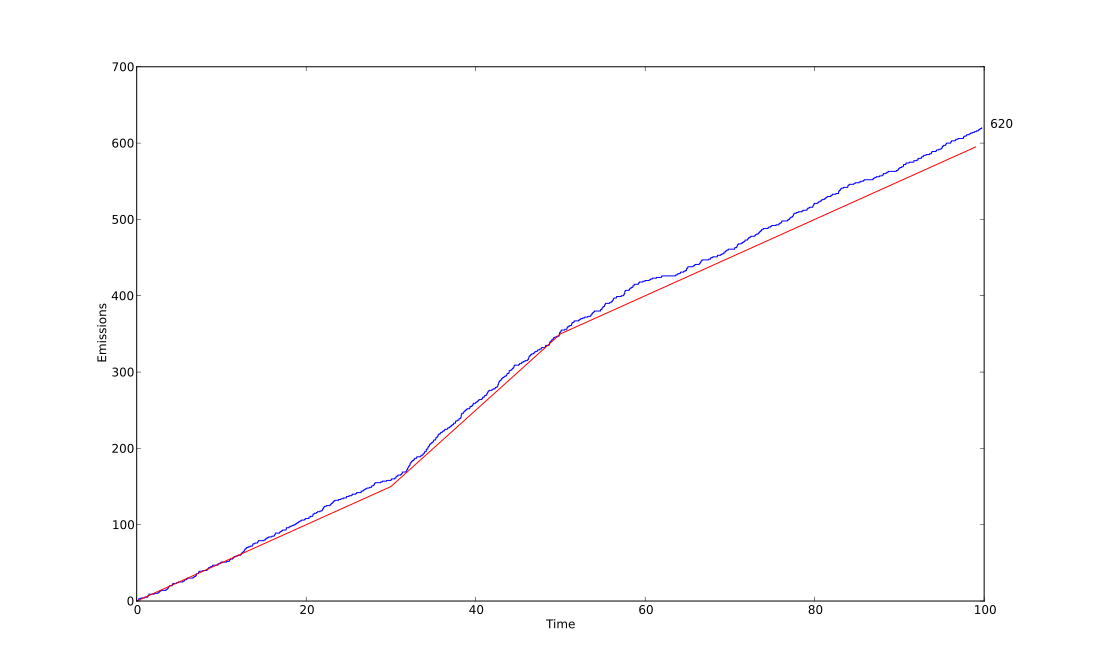
\includegraphics[width = 0.4\textwidth]{./images/integral_fun_1.png}
\caption{A trace of an inhomogeneous Poisson process used to estimate an integral, alongside its true integral, plotted with 620 Poisson emissions}
\label{integral_fun_1}
\end{figure}

\begin{figure}
\centering
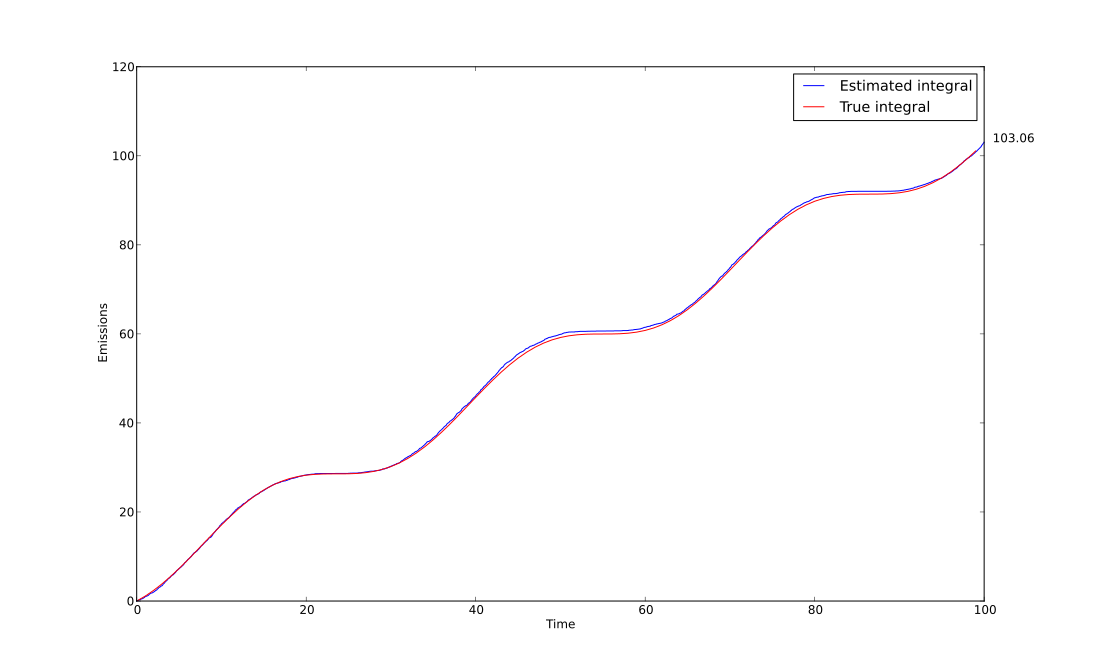
\includegraphics[width = 0.4\textwidth]{./images/integral_fun_2.png}
\caption{A trace of an inhomogeneous Poisson process used to estimate an integral, alongside its true integral, plotted with 5153 Poisson emissions}
\label{integral_fun_2}
\end{figure}

Of course, the actual practicalities of such an algorithm and its relevance to higher-order integrals are yet to be confirmed, though it could be an interesting area for further study.